\chapter{Introduction}

Perudo is a popular dice game that is played all over the world. Perudo is a version played in South America, where it is called many different names such as Dudo, which is Spanish for \textit{I doubt}. It is more well known as Liar's Dice due to the game being called that in ``Pirates of the Caribbean'' movie franchise and the ``Red Dead Redemption'' video game series.

\section{Background}

Perudo is an example of a game with imperfect information. That is, at any point when making a decision we do not know all the information on the board. In this respect, it is similar to Poker, in Perudo we have no idea what the dice that our opponents holds are and in Poker we don't know what cards the opponent is holding. This causes difficulties in detecting possible bluffing. Hence, the optimal strategy can only be estimated with some probabilistic method that heavily depends on the opponents moves.

Perudo, however is not as difficult as Poker as it does not have as large a range of possible card combinations as well as different types of hands. From this one could think of Perudo as a simplified poker.

\section{Rules}

The majority of these games have a common rule set:
\begin{enumerate}
    \item Each player starts with 5 dice.
    \item {\large\epsdice{1}}'s are wildcards, i.e. they count as being every number.
    \item After the previous player bets that there are at least $n$ dice with a certain value, the current player has to raise the bid by raising either the number of dice, the value of the dice or both. In general you can think of each bet as having a score, defined by:
    \begin{equation}
        \label{eq:score}
        s(n, x) = 10n + x
    \end{equation}
    For example, If a player bets that there are at least 2 {\large\epsdice{3}}'s then it would have a value of 23. The current players bet is valid if the score of their bet is greater than the score of the previous bet.
    \item Only the current player may call or raise the bid.
    \item If a player calls, then all dice are revealed and the previous bet is checked. If it was a valid bet the player who has called will loose a die and a new round will start. If the bet was not valid then the previous player looses a die. Whoever looses a die will start the next round.\label{list:call}
    \item A game is finished when there is only one player left with dice.
\end{enumerate}

In Perudo there are 2 special rules that we have to consider.
\paragraph{Palafico}
When a player gets to one die, a special turn (called \textit{Palafico}) occurs. Whatever die value that player begins with cannot be changed. For example, if the \textit{Palafico} player bets that there are 2 {\large\epsdice{3}}'s, then every subsequent bet must raise that bet by saying that there are $n$ {\large\epsdice{3}}'s. A player only gets one \textit{Palafico} round per game. If they survive that round, play goes back to normal.

\paragraph{Aces}
Instead of the usual bidding, players also have the option of trying to predict how many {\large\epsdice{1}}'s there are. In this round, the number of {\large\epsdice{1}}'s predicted has to be \textbf{at least} half the previous amount. For example if the previous bet was 4 {\large\epsdice{3}} then a bet of 2 {\large\epsdice{1}} is valid. Fractions are always rounded up. After a call of \textit{Aces}, the next player may either raise the quantity of {\large\epsdice{1}}'s or they can revert back to the normal method by doubling the quantity of {\large\epsdice{1}}'s called. For example, following a bet of 3 {\large\epsdice{1}}'s, the next bid has to be at least 4 {\large\epsdice{1}}'s or 6 of any other number.

However for this project, we did not include those 2 special rules and only played with the common rule set.

\section{Example of a round}
\begin{figure}[h]
    \centering
    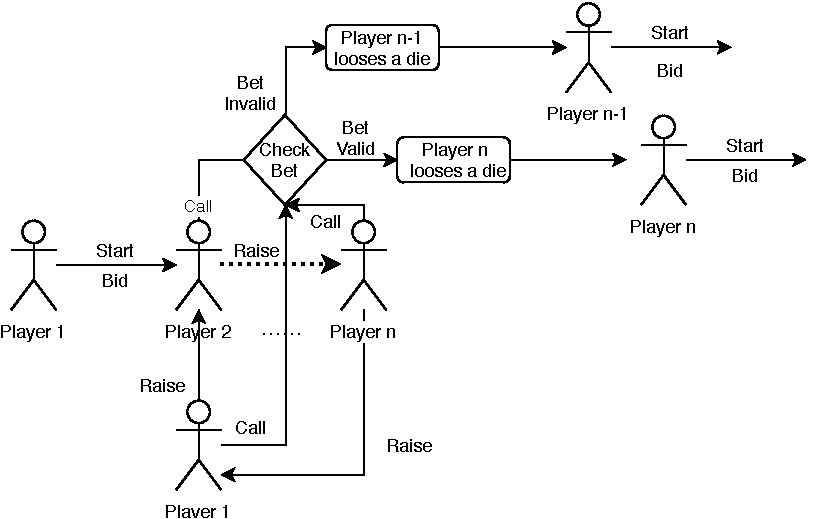
\includegraphics[width=\linewidth,page=1]{flowchart.pdf}
    \caption{Flowchart of a game of Perudo}
    \label{fig:flowcart}
\end{figure}

Using the above flowchart we will play a round of Perudo to get familiar with the rules.

Suppose that each player has the dice in \Cref{table:dicelist} and suppose that the sequence of bets seen in \Cref{fig:round} are placed.

\begin{itemize}
    \item Player 1 starts off the round with by betting 3 {\Large \epsdice{5}}'s.
    \item Player 2 then raises that bet by betting 4 {\Large \epsdice{4}}'s. This is a valid bet because if we look at \Cref{eq:score}, $s(3, 3) = 33 < s(4, 4) = 44$.
    \item Player 3 then raises this bet by betting 5 {\Large\epsdice{4}}'s. This is a valid bet because $s(5, 4) = 54 > s(4, 4) = 44$.
    \item Player 1 calls Player 3's bet. Since there were only 4 {\Large\epsdice{4}}'s, 1 {\Large\epsdice{1}} in Player 1's hand (remember that {\Large\epsdice{1}} are wild cards and count as every number) and 3 {\Large\epsdice{4}}'s in Player 2's hand, Player 3 loses a die.
    \item The round has finished and a new round starts again with Player 3 placing the starting bid.
    \item If Player 3 raised by betting 4 {\Large\epsdice{5}}'s and Player 1 called that bet, Player 1 would have lost a die as there are at least 4 {\Large\epsdice{5}}'s currently in play and a new round starts again with Player 1 starting.
\end{itemize}

\begin{table}[htbp]
    \centering
    \begin{tabular}{ccc}
        % \hline
         Player 1 &Player 2 &Player 3  \\
         \hline
         {\Large\epsdice{1}}{\Large\epsdice{3}}{\Large\epsdice{5}}{\Large\epsdice{5}}{\Large\epsdice{5}}&{\Large\epsdice{1}}{\Large\epsdice{2}}{\Large\epsdice{2}}{\Large\epsdice{4}}{\Large\epsdice{4}}& {\Large\epsdice{2}}{\Large\epsdice{3}}{\Large\epsdice{3}}{\Large\epsdice{5}}{\Large\epsdice{5}}\\
        %  \hline
    \end{tabular}
    \caption{Player's Dice}
    \label{table:dicelist}
\end{table}

\begin{figure}[htbp]
    \centering
    \begin{tikzpicture}[every node/.append style={draw, rounded corners, inner sep=5pt}]
        \node (t1) [rectangle split, rectangle split horizontal, rectangle split parts=2]
        {P1
        \nodepart{two} \Large\epsdice{5}\epsdice{5}\epsdice{5}};

        \node (t2) [rectangle split, rectangle split horizontal, rectangle split parts=2, right of=t1, xshift=2cm]
        {P2
        \nodepart{two} \Large\epsdice{4}\epsdice{4}\epsdice{4}\epsdice{4}};

        \node (t3) [rectangle split, rectangle split horizontal, rectangle split parts=2, right of=t2, xshift=2.5cm]
        {P3
        \nodepart{two} \Large\epsdice{4}\epsdice{4}\epsdice{4}\epsdice{4}\epsdice{4}};

        \node (t4) [rectangle split, rectangle split horizontal, rectangle split parts=2, right of=t3, xshift=2cm]
        {P1
        \nodepart{two} call};

        \node (t5) [rectangle split, rectangle split horizontal, rectangle split parts=2, right of=t4, xshift=2cm]
        {Verify Bet
        \nodepart{two} P3 lied};

        \draw [->, ultra thick] (t1) edge (t2) (t2) edge (t3) (t3) edge (t4) (t4) edge (t5);
    \end{tikzpicture}
    \caption{Round being played}
    \label{fig:round}
\end{figure}


\section{Approach}

Several approaches were used to try and create AI agents. First, a purely probabilistic approach was taken where the agent only considers the probability of the previous players bet when it decides whether it should raise the bet or call. Other approaches that were tried were modifications to this strategy but they took into account information such as the player's current dice and previous bets made. The final approach developed was using the MiniMax algorithm. All agents had 2 parameters that could be tweaked, one for deciding at what the cut-off probability is for deciding if a bet is false and the other parameter that decided what probability the player would bluff with.


To make the code easily extensible, an Object Oriented approach was used throughout the project.

A terminal based application was written that used TCP sockets to communicate with each player to allow them to place bets and receive updates on the game state after each player's turn. This application also allowed a number of games to be played which allows for easy simulation.

\section{Metrics}

The evaluation of the AI agents was done through 2 main methods:

\begin{itemize}
    \item \textbf{Number of wins:} This is the main metric that will be used. It allows us to measure how well the agent performs. By comparing the number of wins each of the approaches had it will allow us to evaluate how good that agent performs.
    \item \textbf{Call Accuracy:} This metric will allows us to find the approach that is the best at calling other players bluff.
\end{itemize}

Using these two metrics will help find the agent that is good at both winning and calling and not just good at one of these tasks.

